\itemhead{数学实验 · 完整实验任务（教材p.73）}{XJ-B1-C03-LAB-P073-Y0145}
\label{XJ-B1-C03-LAB-P073-Y0145}
{\footnotesize 湘教版教材p.73 / PDF第80页 / 数学实验 / 完整实验任务}
\field{原题}{\textbf{用计算机作函数图象和列函数表}
\par 函数的图象能够帮助我们了解函数的性质。我们可以使用计算机技术，根据函数解析式和数据作出函数的图象。使用“超级画板”或其他具有类似功能的软件，在计算机上作函数的图象既快捷又准确。
\par 在右键菜单里单击“函数或参数方程曲线”，在出现的对话框里输入函数表达式“\texttt{x\textasciicircum(1/2)}”，参数范围取 0 到 10，点数取 101，单击“确定”，函数 $y=\sqrt x$ 的图象就出现了。
\bankfig{C03-LAB073}{0.68}
\par 用鼠标在曲线附近单击左键，曲线变色，表示计算机知道你选择了它。执行菜单命令“插入$\mid$表格”，屏幕上就出现了对应的函数表。
\par 这时表上的格子不够，可以用鼠标指着表格按右键，在右键菜单中单击“属性”，打开表格的属性设置对话框，在对话框下部把表格的行数改为 11，列数改为 20，单击“确定”即可。
\par\textit{原页中的软件结果表为操作示例，可在教材p.73核对；本条保留全部实验操作文字与数学表达式，不把软件结果表混作题目条件。}}
\field{参考答案}{实验核查：输入 $y=\sqrt x$，范围 $[0,10]$，101个等距点的横坐标为 $x_k=k/10$（$k=0,\ldots,100$），函数值为 $\sqrt{k/10}$。例如 $(0,0),(1,1),(4,2),(9,3),(10,\sqrt{10})$；图表应一一对应且无负横坐标，不以软件截图代替定义域判断。}
\begin{center}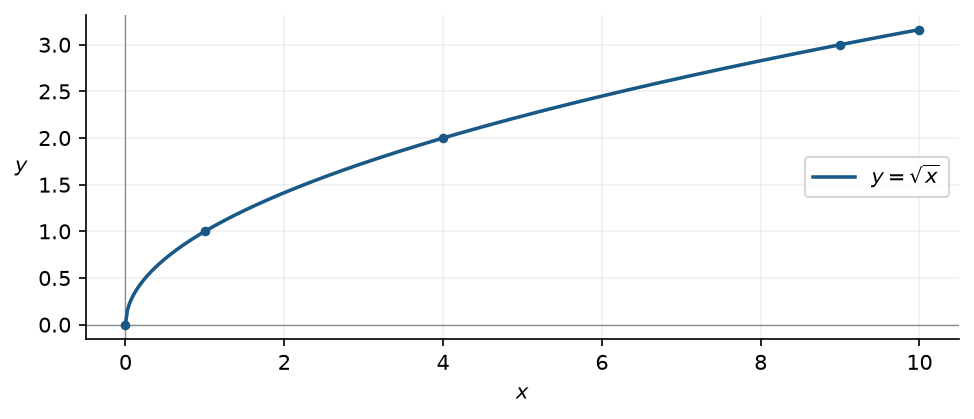
\includegraphics[width=.84\linewidth,height=.38\textheight,keepaspectratio]{figures/C03-LAB073.png}\end{center}
{\small \field{关联知识}{F04 函数三种表示法、图象与读数（教材帮p.85、86、93、94 / PDF94、95、102、103）}
\field{方法与易错点}{把关键点与定义域一起标到图上，逐区间读交点和上下关系。 易错：将示意图预测当事实；把两曲线交点收进严格不等式；折线漏端点。}
\field{答案依据}{答案册未提供本栏目的独立对应答案；依据原题、教材概念补写参考回应。开放性总结不设唯一数值答案。}}
